\begin{figure}[tb]
\centering
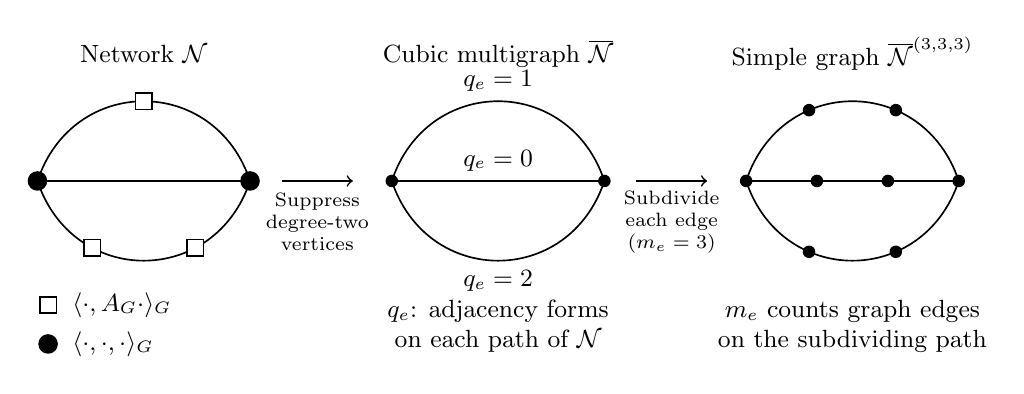
\begin{tikzpicture}[
  x=.9cm,y=.9cm,
  tensor/.style={circle,fill=black,inner sep=2.5pt},
  adjacency/.style={rectangle,draw,fill=white,minimum size=6pt,inner sep=0pt},
  vertex/.style={circle,fill=black,inner sep=1.6pt},
  every node/.style={font=\small},
  line width=.6pt,
]
\node at (1.5,1.8) {Network $\mathcal N$};
\draw (0,0)--(3,0);
\draw (0,0)..controls (.5,1.5) and (2.5,1.5)..(3,0)
  node[pos=.5,adjacency] {};
\draw (0,0)..controls (.5,-1.5) and (2.5,-1.5)..(3,0)
  node[pos=.3,adjacency] {} node[pos=.7,adjacency] {};
\node[tensor] at (0,0) {};
\node[tensor] at (3,0) {};
\node[adjacency] at (.15,-1.75) {};
\node[anchor=west] at (.35,-1.75) {$\langle\cdot,A_G\cdot\rangle_G$};
\node[tensor] at (.15,-2.3) {};
\node[anchor=west] at (.35,-2.3) {$\langle\cdot,\cdot,\cdot\rangle_G$};

\draw[->] (3.45,0)--(4.45,0);
\node[align=center,font=\scriptsize] at (3.95,-.58) {Suppress\\degree-two\\vertices};
\begin{scope}[xshift=4.5cm]
  \node at (1.5,1.8) {Cubic multigraph $\overline{\mathcal N}$};
  \draw (0,0)--(3,0) node[midway,above] {$q_e=0$};
  \draw (0,0)..controls (.5,1.5) and (2.5,1.5)..(3,0)
    node[midway,above] {$q_e=1$};
  \draw (0,0)..controls (.5,-1.5) and (2.5,-1.5)..(3,0)
    node[midway,below] {$q_e=2$};
  \node[vertex] at (0,0) {};
  \node[vertex] at (3,0) {};
  \node[align=center] at (1.5,-2.05) {$q_e$: adjacency forms\\on each path of $\mathcal N$};
\end{scope}

\draw[->] (8.45,0)--(9.45,0);
\node[align=center,font=\scriptsize] at (8.95,-.58) {Subdivide\\each edge\\($m_e=3$)};
\begin{scope}[xshift=9cm]
  \node at (1.5,1.8) {Simple graph $\overline{\mathcal N}^{(3,3,3)}$};
  \draw (0,0)--(3,0) node[pos=.333,vertex] {} node[pos=.667,vertex] {};
  \draw (0,0)..controls (.5,1.5) and (2.5,1.5)..(3,0)
    node[pos=.333,vertex] {} node[pos=.667,vertex] {};
  \draw (0,0)..controls (.5,-1.5) and (2.5,-1.5)..(3,0)
    node[pos=.333,vertex] {} node[pos=.667,vertex] {};
  \node[vertex] at (0,0) {};
  \node[vertex] at (3,0) {};
  \node[align=center] at (1.5,-2.05) {$m_e$ counts graph edges\\on the subdividing path};
\end{scope}
\end{tikzpicture}
\caption{A network, its cubic multigraph, and one simple subdivision.
The path represented by $e$ has $q_e$ adjacency forms and $q_e+1$ edges in $\mathcal N$;
a direct edge has $q_e=0$.
The subdivision on the right is chosen independently of the network paths,
with $m_e=3$ on every edge.
The expansions of $\val_G(\mathcal N)$ and $\hom(\overline{\mathcal N}^{\mathbf m},G)$
use the same coefficients $c_G(\overline{\mathcal N},\ell)$, with weights
$\prod_e\ell(e)^{q_e}$ and $\prod_e\ell(e)^{m_e}$, respectively.
Varying the lengths $m_e\geq3$ determines these coefficients and hence
the network value for every choice of $q_e\geq0$.}
\label{fig:network-subdivision}
\end{figure}
